\section{Modelagem}


\begin{frame}	
	\begin{block}{Amostras viesadas}	
		\begin{itemize}
			\item Precisamos de informação precisa e sem viés para tomarmos boas decisões.
			\item Se você ``cria conhecimento' ou ``toma decisões'' usando informação viesada você não está sendo \# datadriven
			\item A probabilidade de tomar decisões ruins aumenta... e decisões ruins costumam ser caras...
		\end{itemize}		
	\end{block}
\end{frame}

\begin{frame}	
	\begin{block}{processo de KDD}	
		\begin{figure}[!htb]
			\centering	  				
			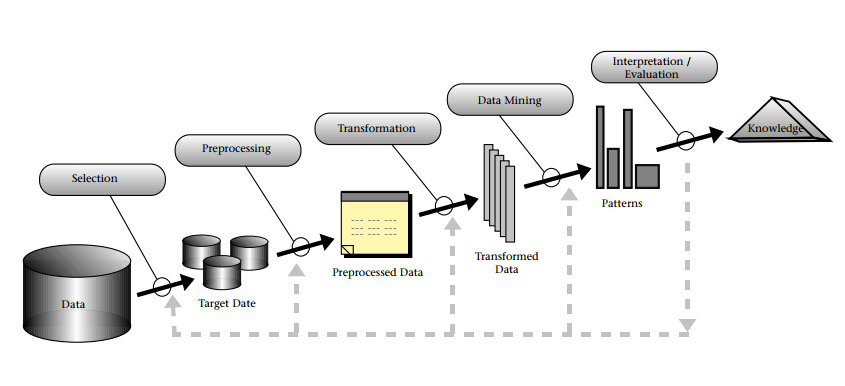
\includegraphics[height=5cm, width = 12cm]{./pic/kddprocess.jpg}
			\caption{Processo de KDD}
			\label{fig_kdd_process}
		\end{figure}
		\begin{itemize}
			\item Se você cometer um erro durante a etapa de: ``seleção'' os passos seguintes e suas conclusões estarão erradas.
		\end{itemize}
	\end{block}
\end{frame}

\begin{frame}	
	\begin{block}{Amostragem 101}	
		\begin{figure}[!htb]
			\centering	  				
			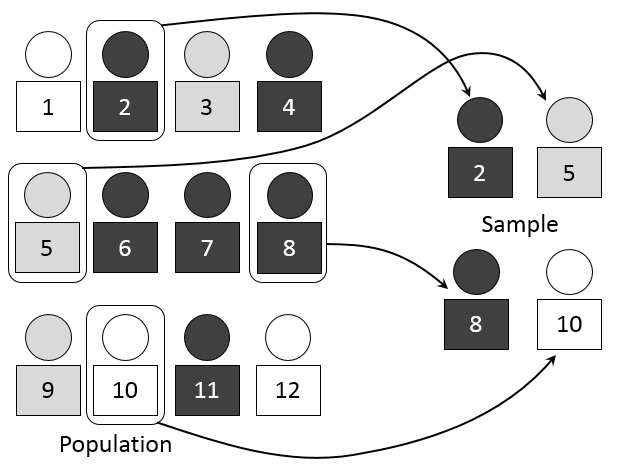
\includegraphics[height=5cm, width = 12cm]{./pic/sampling.png}
			\caption{Overview de amostragem}
			\label{fig_sampling}
		\end{figure}
		\begin{itemize} 
			\item O subconjunto (amostra) de elementos deve ser representativa da população.
		\end{itemize}
	\end{block}
\end{frame}

\begin{frame}	
	\begin{block}{Bias de auto seleção}	
		\begin{itemize} 
			\item Suponha um estudo estatístico sobre detalhes íntimos da sexualidade de estudantes em universidades. Algumas pesssoas provavelmente vão mentir.
			\item Uma pesquisa online sobre quem gosta de usar computador.
			\item Em ambos as pessoas selecionadas vão terão seus comportamentos diferentes da população geral.
		\end{itemize}
	\end{block}
\end{frame}


\begin{frame}	
	\begin{block}{Undercoverage Bias}	
		\begin{itemize} 
			\item Digest em 1936 fez uma pesquisa eleitoral que previa vitória larga do candidato Lando em relação ao candidato Roosevelt. Roosevelt ganhou com uma margem larga, a pesquisa era feita por telefone, na época pessoas pobres (maioria da população que era a favor de Roosevelt) não tinha telefone. Essa foi uma das causas do erro estatístico.
		\end{itemize}
	\end{block}
\end{frame}

\begin{frame}	
	\begin{block}{Survivorship Bias}	
		\begin{itemize} 
			\item Ocorre quando as observações estudadas no fim da investigação são não aleatórias em comparação as presentes no começo da observação.		
		\end{itemize}
	\end{block}
\end{frame}


\begin{frame}	
	\begin{block}{Survivorship Bias}	
		\begin{itemize} 
			\item Exemplo da segunda guerra mundial (tiros em avião)
		\end{itemize}
	\end{block}
\end{frame}


\begin{frame}	
	\begin{block}{Engenharia de features}
		\begin{itemize}
			\item Modelos usam muitas variáveis para tomar decisões
			\item Encontrar boas variáveis é parte fundamental para um modelo
			\item Citar exemplo de variáveis de transações financeiras
			\item Citar exemplo de variáveis de pagamento de assinaturas
			\item Citar exemplo de um classificador de brasileiros e peruanos			
		\end{itemize}		
	\end{block}
\end{frame}


\begin{frame}	
	\begin{block}{Modelos}	
			\begin{figure}[!htb]
			\centering	  				
			
\includegraphics[height=6cm, width = 10cm]{./pic/AI.png}
			\caption{Brincadeira, cada modelo trabalha internamente de uma forma distinta!}
			\label{fig_brincadeira}
		\end{figure}	
	\end{block}
\end{frame}

\begin{frame}	
	\begin{block}{Modelos}	
		\begin{itemize}
			\item Modelos tomam decisões baseados em diversas variáveis para, entre outras coisas, classificar dados
			\item Quem são peruanos e quem são brasileiros nessa sala?
			\item Há modelos para classificar em duas classes ou mais.
		\end{itemize}			
		\begin{figure}[!htb]
			\centering	  				
			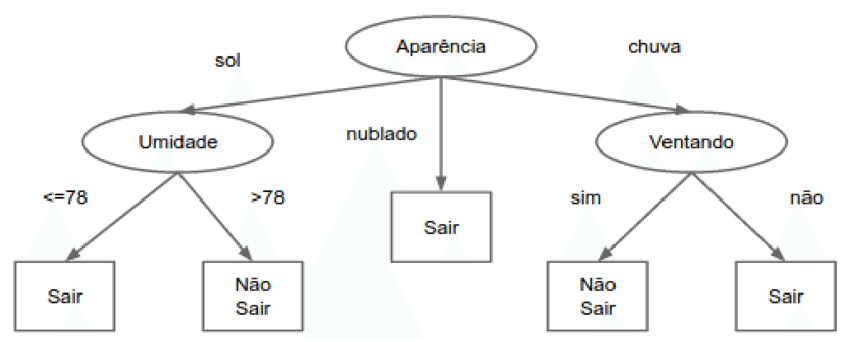
\includegraphics[height=4cm, width = 10cm]{./pic/arvore.png}
			\caption{Exemplo de árvore de decisão para sair de casa}
			\label{fig_Arvore}
		\end{figure}	
	\end{block}
\end{frame}


\begin{frame}	
	\begin{block}{Ferramentas}	
		\begin{itemize}
			\item Na teoria pode-se usar qualquer linguagem de programação para trabalhar com Data Science
			\item Na prática usa-se, majoritariamente, a plataforma R e a linguagem python (com alguns pacotes científicos)
			\item http://scikit-learn.org/stable/  (biblioteca Python)
			\item https://www.r-bloggers.com (blog de plataforma científica)
		\end{itemize}		
	\end{block}
\end{frame}

\begin{frame}	
	\begin{block}{Treinamento}	
		\begin{itemize}
			\item O processo de treinamento é único para cada modelo mas a forma como se treina um modelo é parecida
			\item Os dados são dividos em treino (70\%) e teste (30\%)
			\item O conjunto de treino é apresentado ao modelo com os rótulos de cada observação
			\item Tipicamente usa-se uma validação cruzada para treinar o modelo
		\end{itemize}		
	\end{block}
\end{frame}

\begin{frame}	
	\begin{block}{Validação}	
		\begin{itemize}
			\item O modelo é validado com o conjunto de teste, o qual não deve exibir os rótulos para o modelo
			\item Alguma métrica de validação de modelos é usada, por exemplo, precisão $\dfrac{VP}{VP + FP}$
		\end{itemize}
				\begin{figure}[!htb]
			\centering	  				
			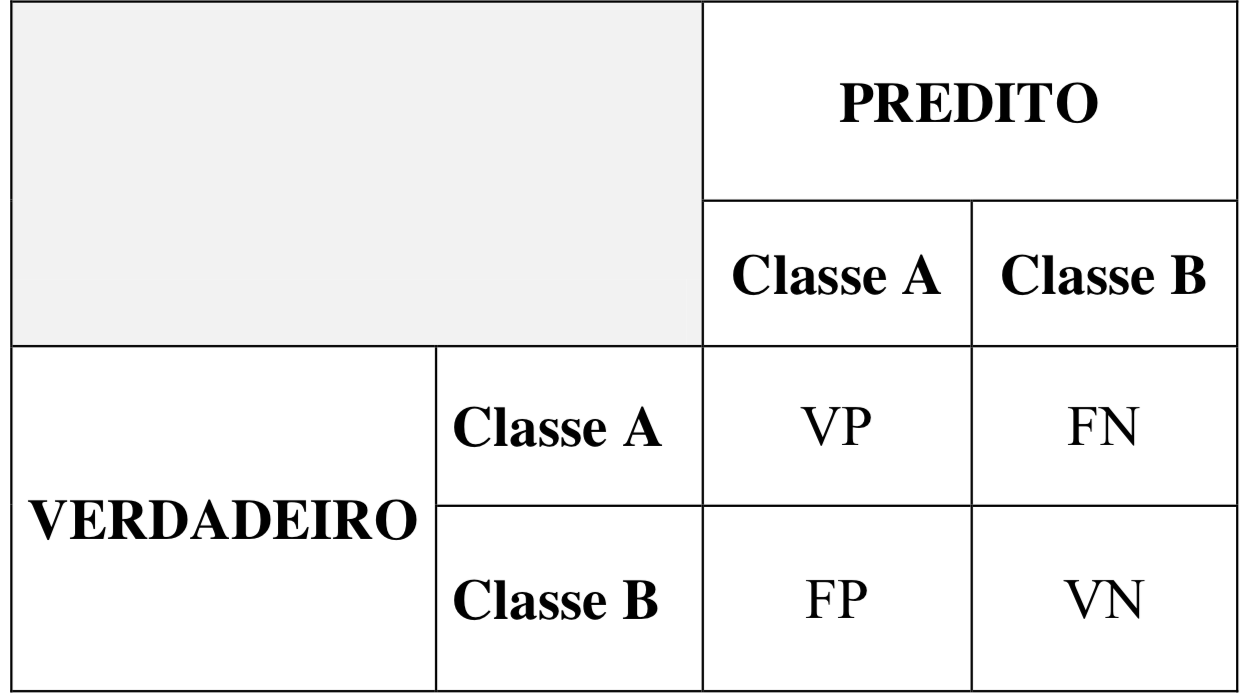
\includegraphics[height=4cm, width = 10cm]{./pic/matrizConfusao.png}
			\caption{Obtido no link: \href{http://www.scielo.br/pdf/eagri/v33n6/19.pdf}{Scielo} }
			\label{fig_matriz_confusao}
		\end{figure}	
	\end{block}
\end{frame}


% Colocar metricas aqui
\begin{frame}	
	\begin{block}{Métricas}	
		\begin{align*}
			\textrm{Precision} &= \frac{TP}{TP + FP} \\ \\
			\textrm{Recall} &= \frac{TP}{TP + FN} \\ \\
			\textrm{F1} &= 2 \left( \frac{  \textrm{Precision} * \textrm{Recall}    }{\textrm{Precision} + \textrm{Recall} } \right)
		\end{align*}
	\end{block}
\end{frame}


\begin{frame}	
	\begin{block}{Métricas de uma forma visual}	
		\begin{figure}[!htb]
			\centering	  				
			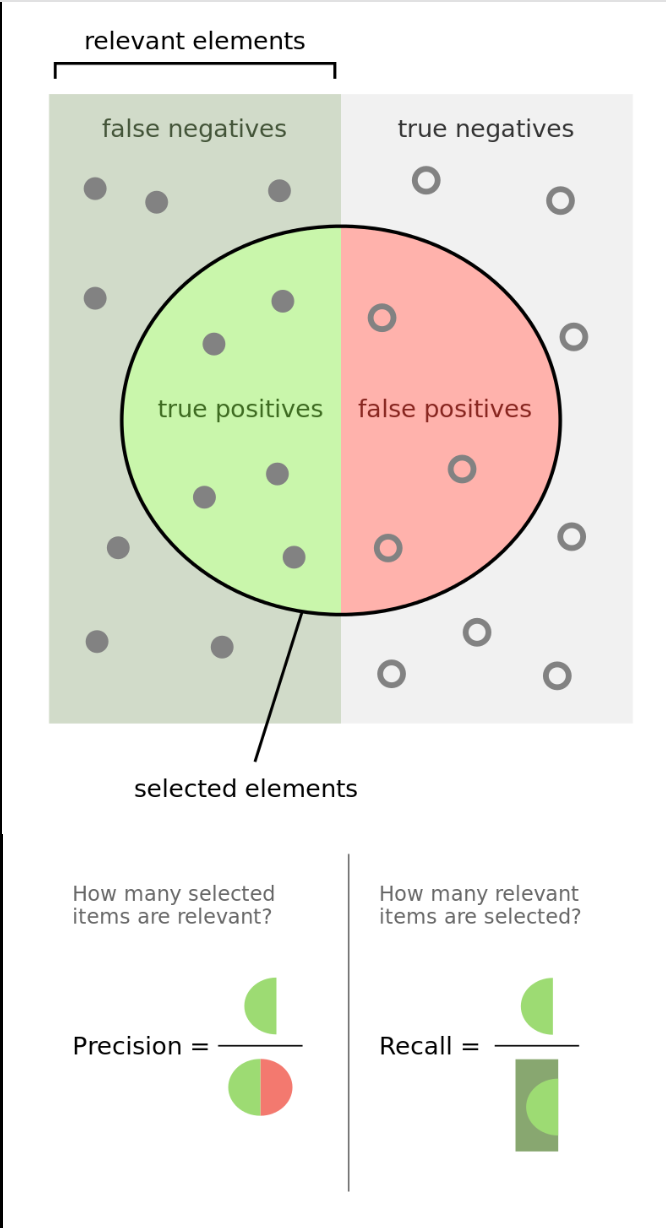
\includegraphics[height=7cm, width = 8cm]{./pic/OverviewMetricas.png}
			\caption{Métricas de uma forma visual}
			\label{fig_metricas_visual}
		\end{figure}
	\end{block}
\end{frame}


\begin{frame}	
	\begin{block}{Gráficos}	
		\begin{itemize}
			\item Curva ROC (``True Positive Rate vs. False Positive Rate'')
			\item AuC (Área sobre a curva ROC)
		\end{itemize}		
	\end{block}
\end{frame}


\begin{frame}	
	\begin{block}{Exemplo ROC e AUC}	
		\begin{figure}[!htb]
			\centering	  				
			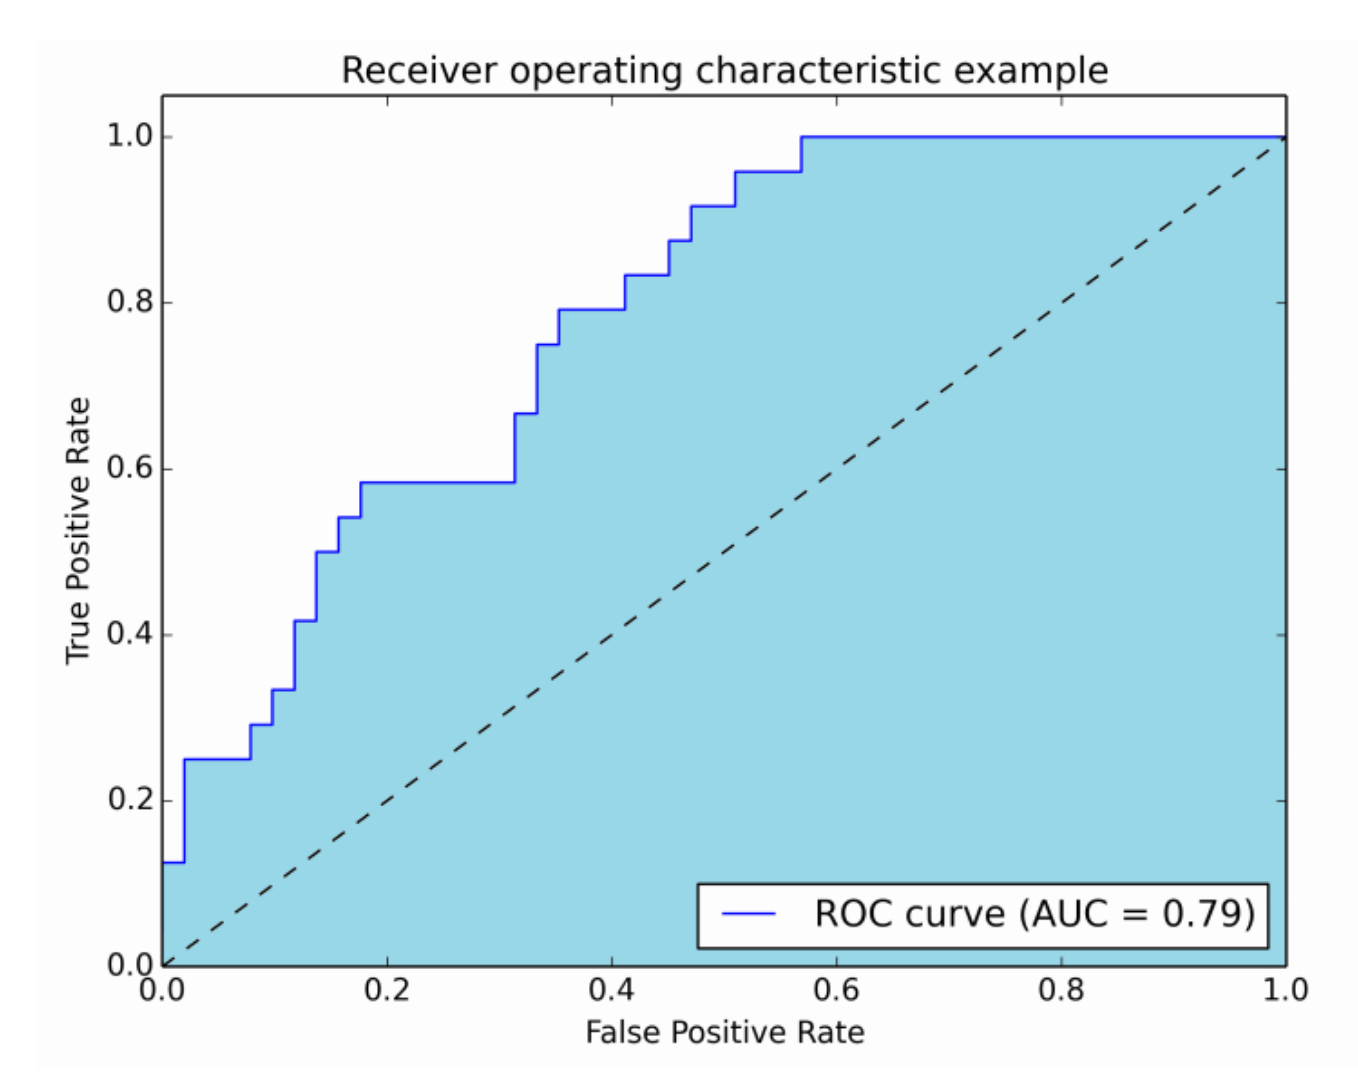
\includegraphics[height=7cm, width = 10cm]{./pic/Auc.png}
			\caption{Exemplo ROC e AUC}
			\label{fig_roc_auc}
		\end{figure}
	\end{block}
\end{frame}

\begin{frame}	
	\begin{block}{Comparação de modelos}	
		\begin{figure}[!htb]
			\centering	  				
			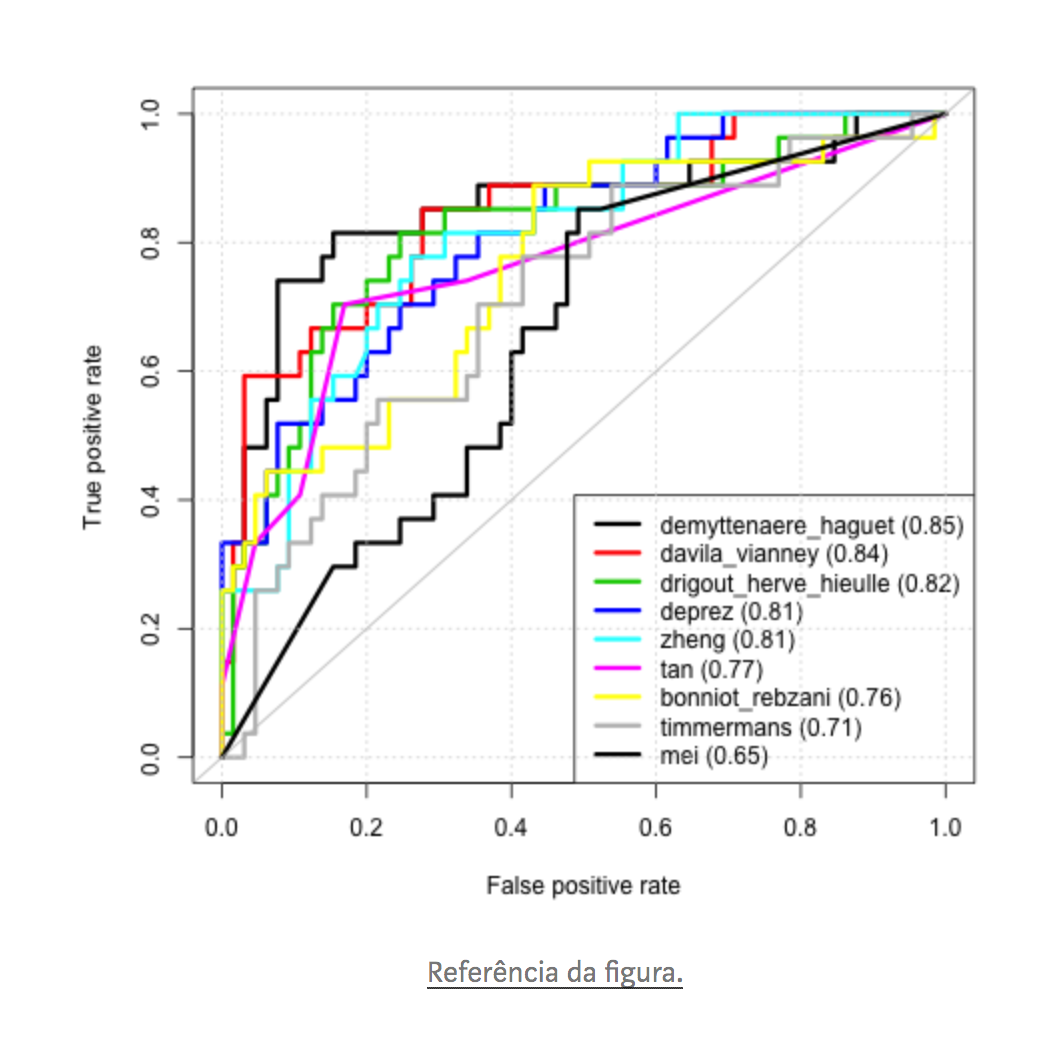
\includegraphics[height=7cm, width = 12cm]{./pic/MultiROC.png}
			\caption{Comparação de modelos}
			\label{fig_comparacao_modelos}
		\end{figure}
	\end{block}
\end{frame}


% Colocar resumo dos algoritmos
\begin{frame}	

		\begin{figure}
			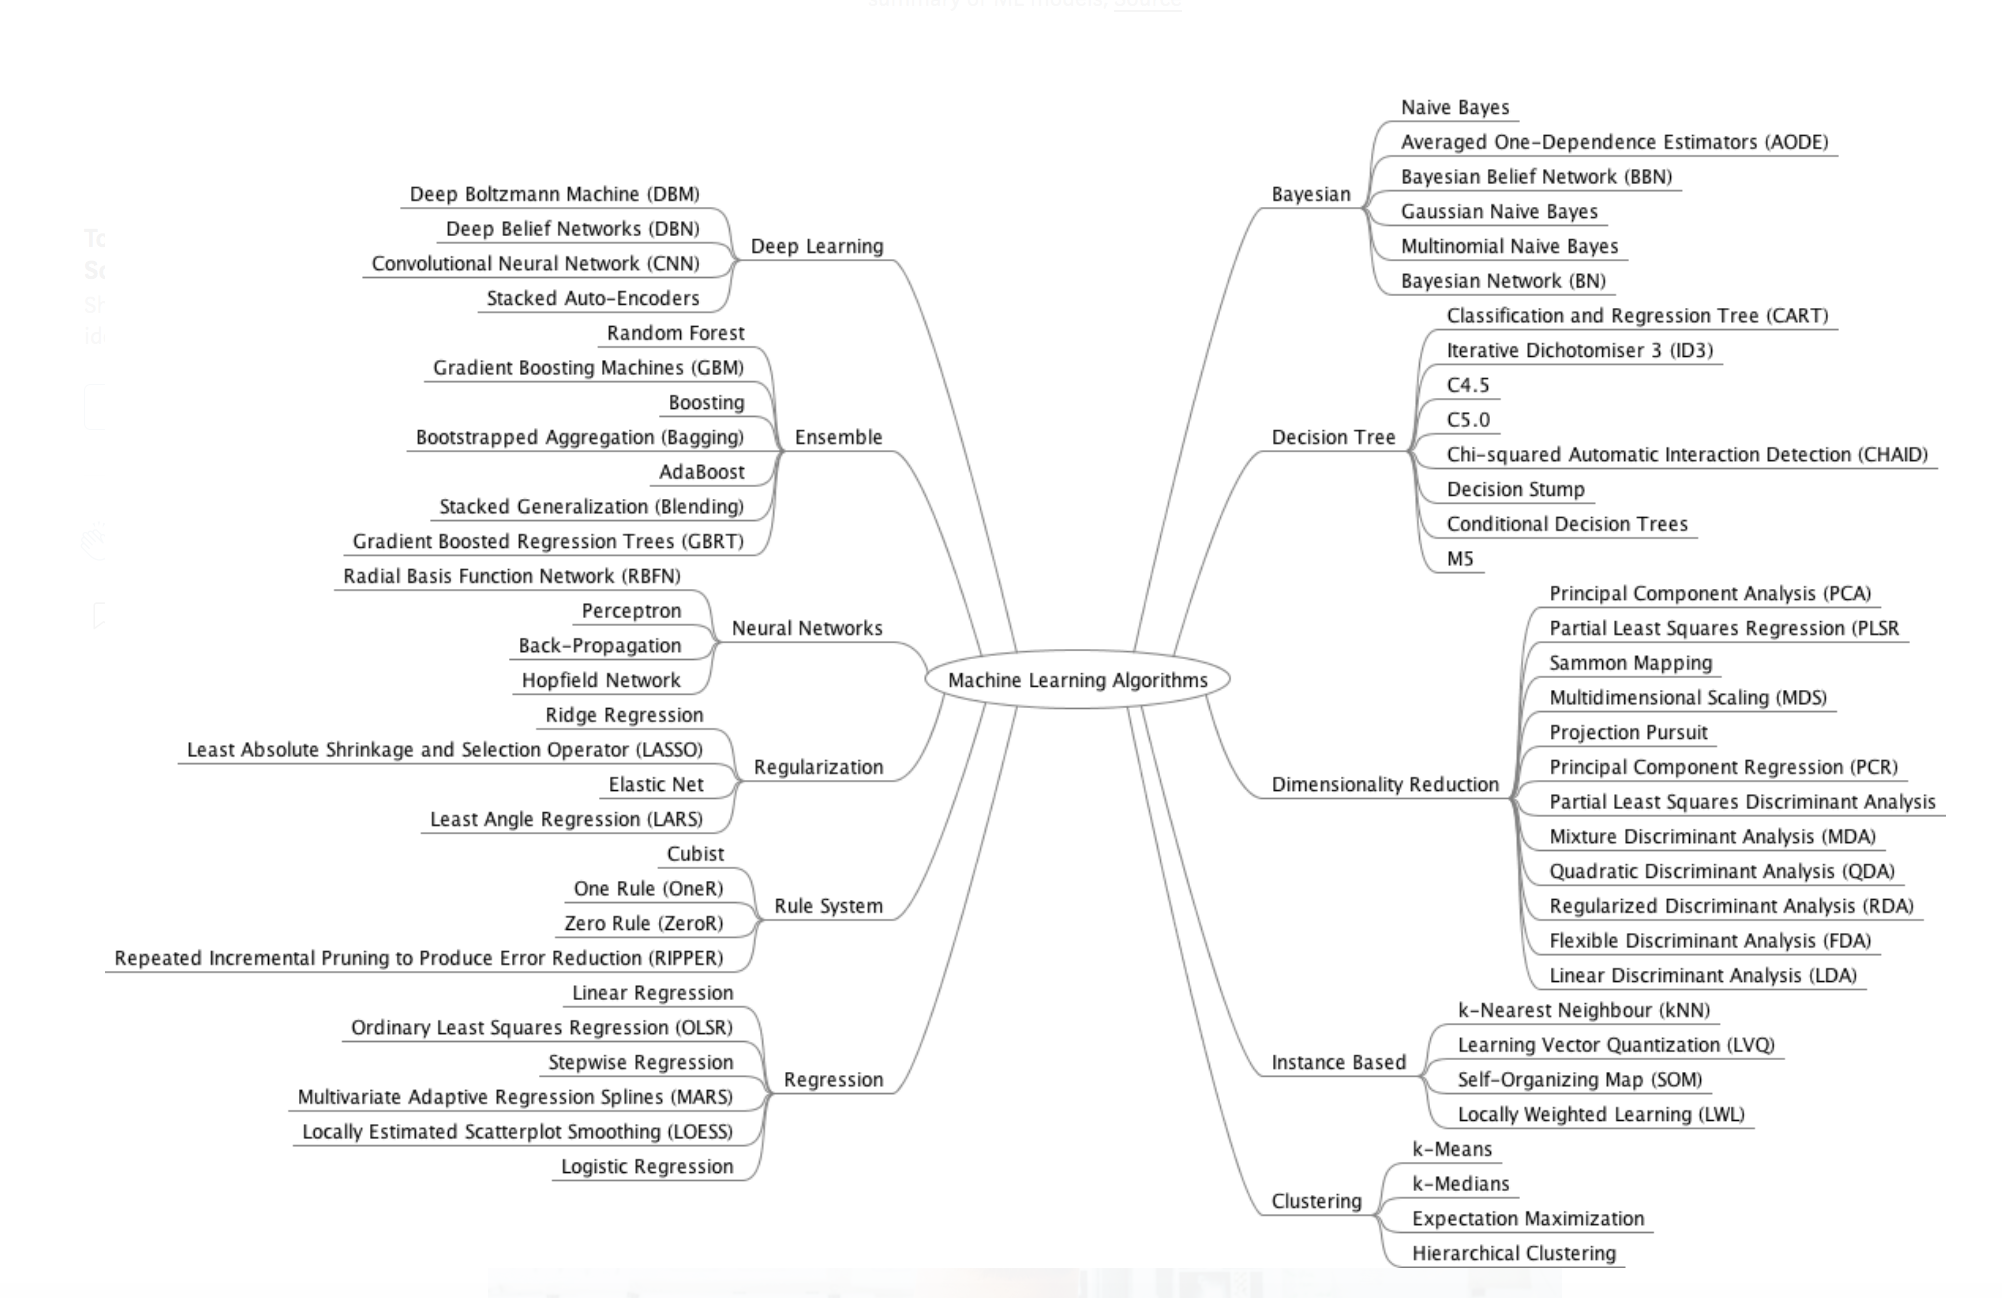
\includegraphics[height=8.5cm, width = 12cm]{./pic/algoritmos1.png}
			\label{fig_modelos}
		\end{figure}

\end{frame}

\begin{frame}	
	\begin{block}{Exemplos de modelos}	
		\begin{figure}[!htb]
			\centering	  				
			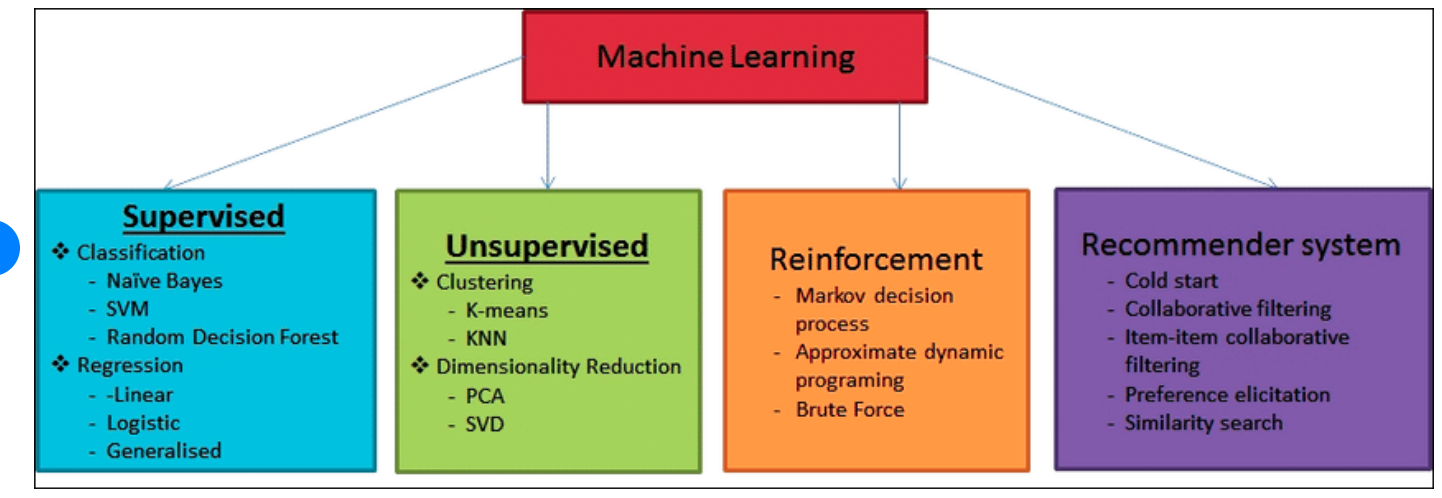
\includegraphics[height=6cm, width = 10cm]{./pic/algoritmos2.png}
			\caption{Exemplos de modelos 2}
			\label{fig_modelos}
		\end{figure}
	\end{block}
\end{frame}

\begin{frame}	
	\begin{block}{Exemplos de modelos}	
		\begin{figure}[!htb]
			\centering	  				
			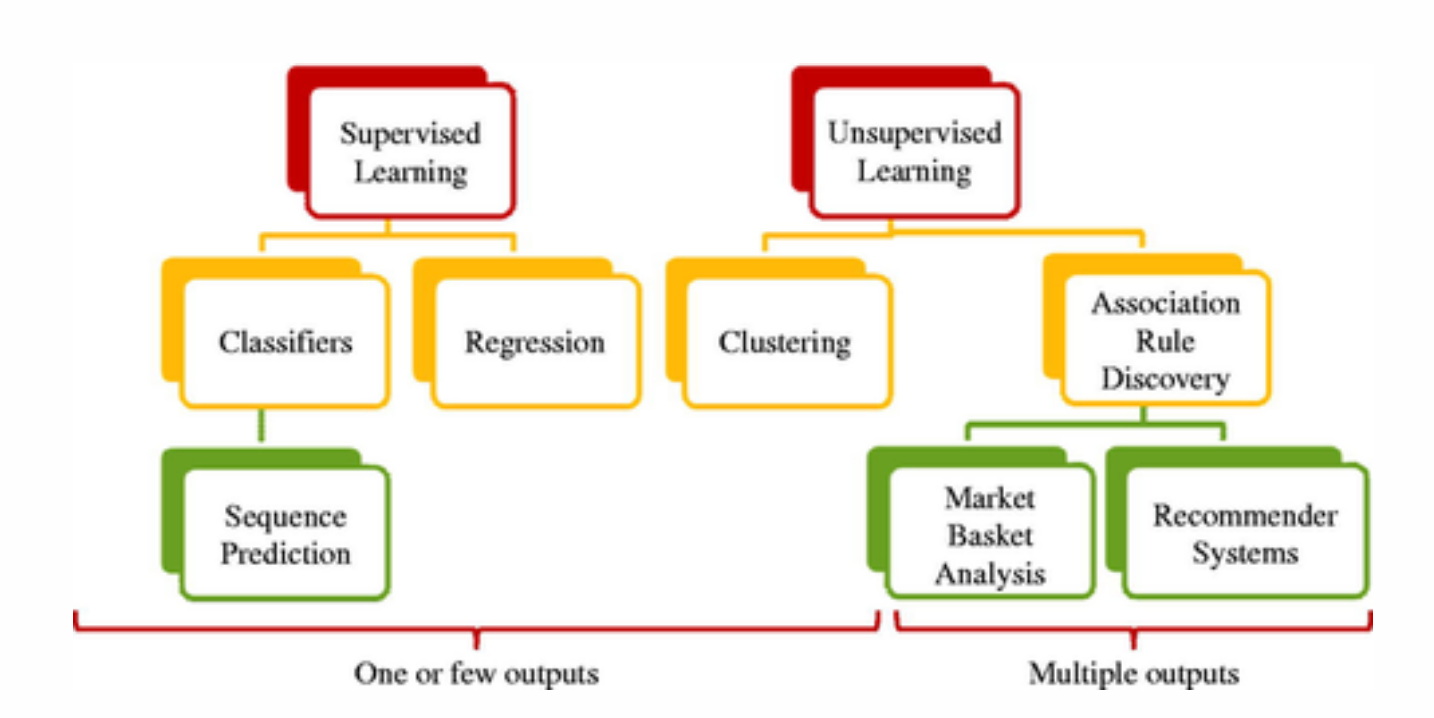
\includegraphics[height=5cm, width = 10cm]{./pic/algoritmos3.png}
			\caption{Exemplos de modelos 3}
			\label{fig_modelos}
		\end{figure}
	\end{block}
\end{frame}

%https://machinelearningmastery.com/a-tour-of-machine-learning-algorithms/
\begin{frame}	
	\begin{block}{Modelos baseados em árvore}	
		\begin{figure}[!htb]
			\centering	  				
			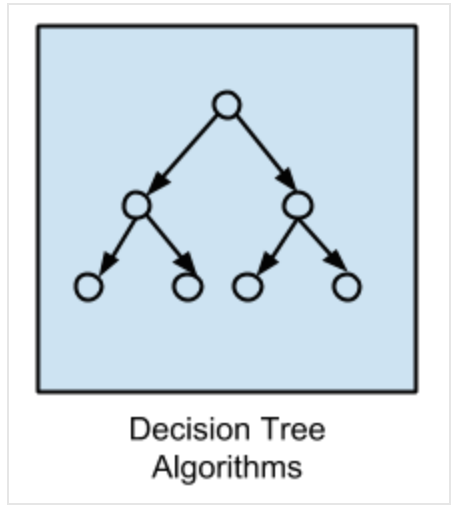
\includegraphics[height=5cm, width = 10cm]{./pic/arvoreResumo.png}
			\caption{Modelos baseados em árvore}
			\label{fig_modelos}
		\end{figure}
	\end{block}
\end{frame}


\begin{frame}	
	\begin{block}{Sobre esses modelos}	
		\begin{itemize}
			\item Treina o modelo usando os valores dos dados apresentados
			\item Cada nós da árvore é uma decisão tomada, encontrar os nós é o trabalho do treinamento
			\item CART, $C4.5$, $C5.0$, $CHAID$ são exemplos de algoritmos baseados em árvore
		\end{itemize}		
	\end{block}
\end{frame}


\begin{frame}	
	\begin{block}{Modelos baseados em regressão}	
		\begin{figure}[!htb]
			\centering	  				
			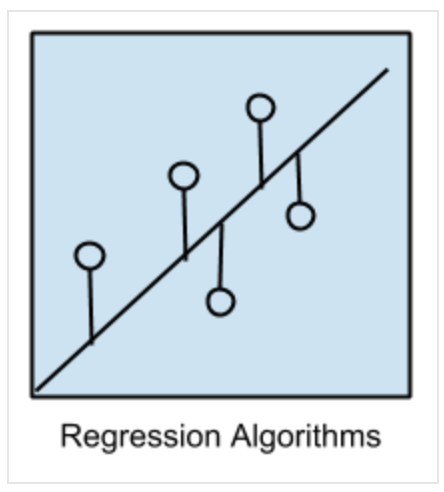
\includegraphics[height=5cm, width = 10cm]{./pic/regressao.png}
			\caption{Modelos baseados em regressão}
			\label{fig_modelos}
		\end{figure}
	\end{block}
\end{frame}


\begin{frame}	
	\begin{block}{Sobre esses modelos}	
		\begin{itemize}
			\item Regressão consiste em treinar um modelo que se adapta numéricamente aos dados de forma iterativa
			\item A cada iteração reduzimos o erro
			\item Reg. Linear, Logistica, OLSR, MARS são exemplos de algoritmos de regressão.
		\end{itemize}
	\end{block}
\end{frame}


\begin{frame}	
	\begin{block}{Modelos baseados em Instância}	
		\begin{figure}[!htb]
			\centering	  				
			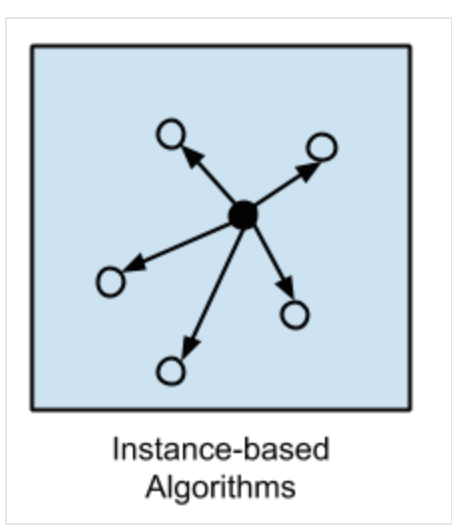
\includegraphics[height=5cm, width = 10cm]{./pic/instance.png}
			\caption{Modelos baseados em Instância}
			\label{fig_modelos}
		\end{figure}
	\end{block}
\end{frame}


\begin{frame}	
	\begin{block}{Sobre esses modelos}	
		\begin{itemize}
			\item Constroem uma base de conhecimento sobre os pontos dos dados
			\item Novos pontos são comparados com a base usando uma métrica de distância
			\item A menor distância é usada para classificar esses pontos
			\item KNN, LVQ, SOM, SVM são exemplos de algoritmos
		\end{itemize}
	\end{block}
\end{frame}


\begin{frame}	
	\begin{block}{Modelos baseados em regularização}	
		\begin{figure}[!htb]
			\centering	  				
			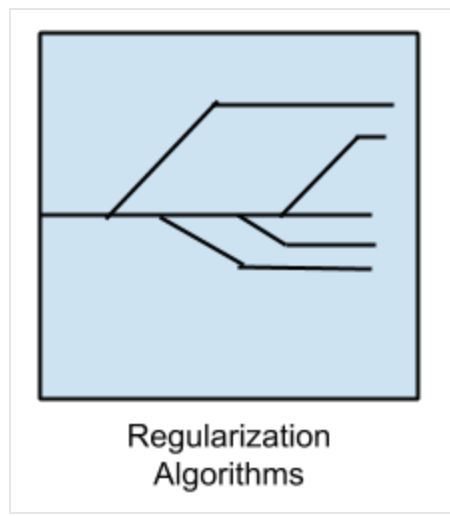
\includegraphics[height=5cm, width = 10cm]{./pic/penalizacao.png}
			\caption{Modelos baseados em regularização}
			\label{fig_modelos}
		\end{figure}
	\end{block}
\end{frame}


\begin{frame}	
	\begin{block}{Sobre esses modelos}	
		\begin{itemize}
			\item Extensão de técnicas de regressão
			\item Usa um fator de regularização (modelos mais complexos são penalizados)
			\item Tenta evitar o overfitting
			\item Reg. Ridge, LASSO são exemplos de algoritmos 
		\end{itemize}
	\end{block}
\end{frame}

\begin{frame}	
	\begin{block}{Modelos baseados em Bayes}	
		\begin{figure}[!htb]
			\centering	  				
			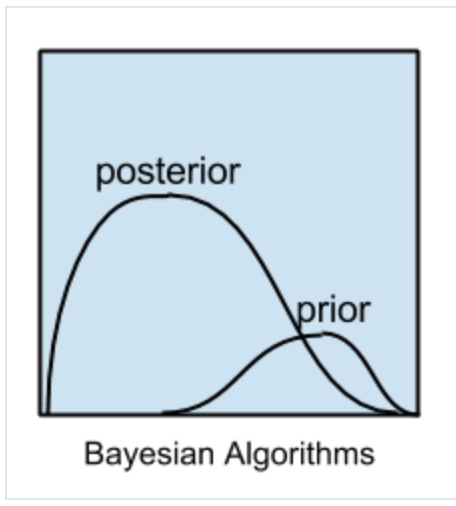
\includegraphics[height=5cm, width = 10cm]{./pic/bayes.png}
			\caption{Modelos baseados em Bayes}
			\label{fig_modelos}
		\end{figure}
	\end{block}
\end{frame}


\begin{frame}	
	\begin{block}{Sobre esses modelos}	
		\begin{itemize}
			\item Aplicam o teorema de Bayes para predizer
			\item Tipicamente necessitam conhecimento prévio das probabilidades da classe target
			\item Naive Bayes, Bayesian Network (BN), Multinomial Naive Bayes  são exemplos de algoritmos 
		\end{itemize}
	\end{block}
\end{frame}


\begin{frame}	
	\begin{block}{Modelos baseados em Agrupamento}	
		\begin{figure}[!htb]
			\centering	  				
			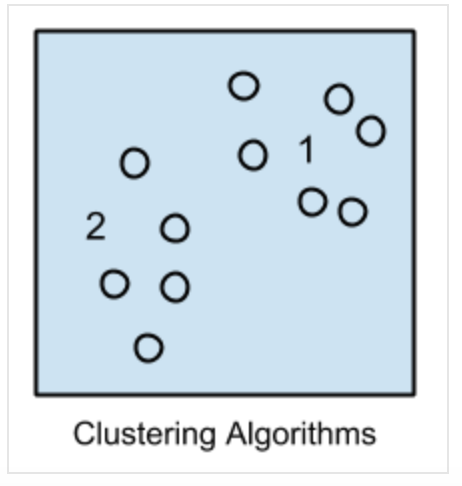
\includegraphics[height=5cm, width = 10cm]{./pic/cluster.png}
			\caption{Modelos baseados em Agrupamento}
			\label{fig_modelos}
		\end{figure}
	\end{block}
\end{frame}


\begin{frame}	
	\begin{block}{Sobre esses modelos}	
		\begin{itemize}
			\item Usam alguma métrica de distância para tentar organizar os dados em agrupamentos
			\item Há técnicas baseadas em centróides, hierárquicas, densidade entre outras
			\item k-Means, k-Medians, CLARA, CLARANS, AGNES, DIANA, DBSCAN  são exemplos de algoritmos 
		\end{itemize}
	\end{block}
\end{frame}


\begin{frame}	
	\begin{block}{Modelos baseados em regras de associação}	
		\begin{figure}[!htb]
			\centering	  				
			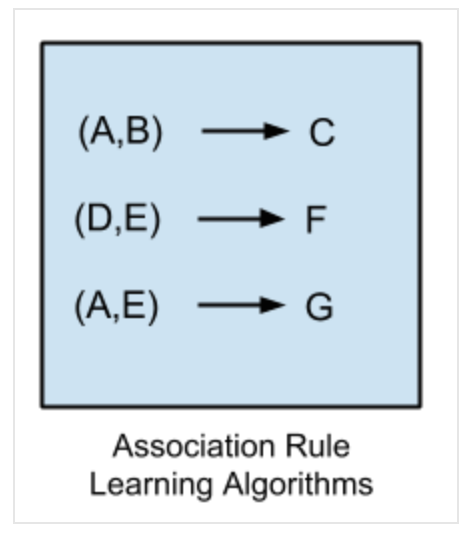
\includegraphics[height=5cm, width = 10cm]{./pic/regrasAssociacao.png}
			\caption{Modelos baseados em associação}
			\label{fig_modelos}
		\end{figure}
	\end{block}
\end{frame}


\begin{frame}	
	\begin{block}{Sobre esses modelos}	
		\begin{itemize}
			\item Extraem regras que expliquem melhor as relações  entre variáveis
			\item A famosa ``análise de carrinho de compra''
			\item Apriori, Eclat são exemplos de algoritmos 
		\end{itemize}
	\end{block}
\end{frame}



\begin{frame}	
	\begin{block}{Modelos baseados em redes neurais}	
		\begin{figure}[!htb]
			\centering	  				
			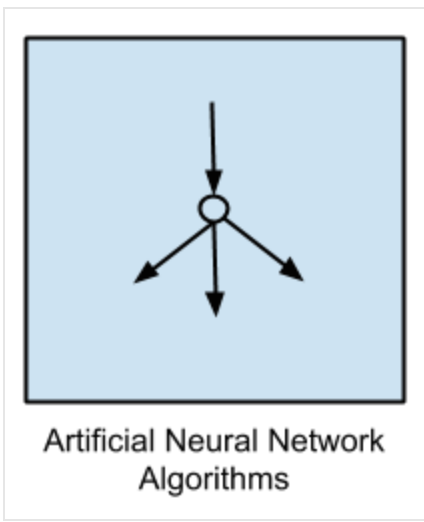
\includegraphics[height=5cm, width = 10cm]{./pic/redeneural.png}
			\caption{Modelos baseados em redes neurais}
			\label{fig_modelos}
		\end{figure}
	\end{block}
\end{frame}


\begin{frame}	
	\begin{block}{Sobre esses modelos}	
		\begin{itemize}
			\item Inspirados em neurônios biológicos
			\item Consistem em encontrar pesos para a rede neural
			\item Perceptron, MLP, Hopfield Network são exemplos de algoritmos 
		\end{itemize}
	\end{block}
\end{frame}


\begin{frame}	
	\begin{block}{Modelos baseados em Deep Learning}	
		\begin{figure}[!htb]
			\centering	  				
			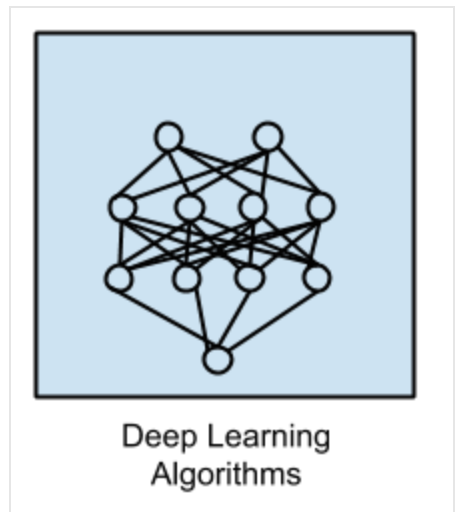
\includegraphics[height=5cm, width = 10cm]{./pic/deepLearning.png}
			\caption{Modelos baseados em Deep Learning}
			\label{fig_modelos}
		\end{figure}
	\end{block}
\end{frame}


\begin{frame}	
	\begin{block}{Sobre esses modelos}	
		\begin{itemize}
			\item Evolução das redes neurais
			\item Convolutional Neural Network (CNN), Long Short-Term Memory Networks (LSTMs) são exemplos de algoritmos 
		\end{itemize}
	\end{block}
\end{frame}


\begin{frame}	
	\begin{block}{Modelos baseados em redução de dimensionalidade}	
		\begin{figure}[!htb]
			\centering	  				
			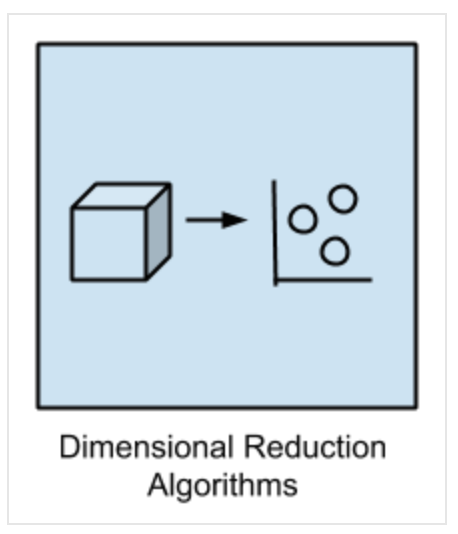
\includegraphics[height=5cm, width = 10cm]{./pic/reducao.png}
			\caption{Modelos baseados em redução de dimensionalidade}
			\label{fig_modelos}
		\end{figure}
	\end{block}
\end{frame}


\begin{frame}	
	\begin{block}{Sobre esses modelos}	
		\begin{itemize}
			\item Explora a estrutura dos dados para tentar remover features que não são importantes 
			\item São não supervisionados
			\item PCA, SVD, LDA, FDA são exemplos de algoritmos
		\end{itemize}
	\end{block}
\end{frame}


\begin{frame}	
	\begin{block}{Modelos baseados em ensemble}	
		\begin{figure}[!htb]
			\centering	  				
			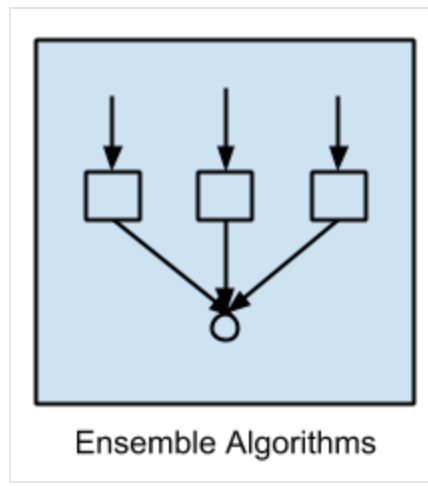
\includegraphics[height=5cm, width = 10cm]{./pic/ensemble.png}
			\caption{Modelos baseados em ensemble}
			\label{fig_modelos}
		\end{figure}
	\end{block}
\end{frame}


\begin{frame}	
	\begin{block}{Sobre esses modelos}	
		\begin{itemize}
			\item Modelos compostos de outros modelos treinados de forma independente
			\item As predições são combinadas de alguma maneira
			\item Boost, Random Forest, Rotation Forest, Xgboost  são exemplos de algoritmos
		\end{itemize}
	\end{block}
\end{frame}

% Resumir o boost


%\begin{frame}
%	\begin{block}{Hands on}	
%		\begin{itemize}
%			\item Treinar modelo em R com os alunos
%			\item Treinar modelo em PYTHON com os alunos
%		\end{itemize}		
%	\end{block}
%\end{frame}

